
\section{Experiments}\label{sec:boa-expe}
In \cref{sec:boa-reconstruction} and \cref{sec:boa-metric-perf}, we explore the limits of BoA \textit{w.r.t.} input data.
In \cref{sec:boa-real-world-expe}, we reproduce the experiments from~\cite{fca2vec:2019:durrschnabel} on real-world data.
%In this section we explore the limits of our model with regards to the input data.
%We first examine the scalability of the approach, then we evaluate the sensitivity of the approach to perturbation of the data.
All the experiments described in \cref{sec:boa-reconstruction} and \cref{sec:boa-metric-perf} are performed on randomly generated data to control the of the evaluation process.
%(in terms of performance)

    
\subsection{Reconstruction Performance}\label{sec:boa-reconstruction}
To assess the reconstruction performance of the BoA auto-encoder, we use the \textit{area under the receiver operating characteristic curve} (AUC ROC).
It allows us to determine whether the BoA has a good predictive capacity and, similarly to the F1 measure, AUC ROC gives a general account of performance. %, as the receiver operating characteristics curve depends on precision and recall.
%AUC ROC goes from 0 to 1, with results close to $0.5$ corresponding to poor predictive performance and those closer to $1$ correspond to better models.
To determine if the results are significantly different, we use Student t-test on means.
The results are presented in \cref{fig:limits}.

\begin{figure}
\centering
\subcaptionbox{Impact of the density, from 0.1 to 0.9, 100 samples per density.\label{fig:limits_density}}
    {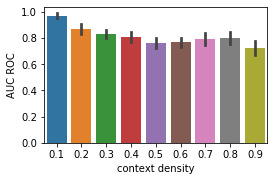
\includegraphics[width=.48\textwidth, height=4cm, keepaspectratio]{Figures/Ch2/limits_densities.png}  }
\subcaptionbox{Impact of the size, from 5 to 500 objects and attributes, 20 samples per size.\label{fig:limits_size}}
    {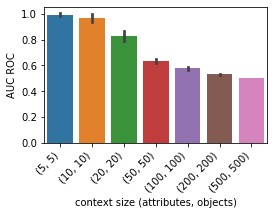
\includegraphics[width=.48\textwidth, height=4cm, keepaspectratio]{Figures/Ch2/limits_size.png}  }
\subcaptionbox{Impact of the concept number, for 200 sample with 20 objects and attributes. The blue line is the general tendency when rounding the concept number to 50.\label{fig:limits_concepts}}
    {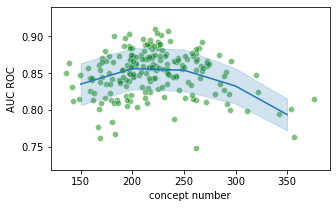
\includegraphics[width=.48\textwidth, height=4cm, keepaspectratio]{Figures/Ch2/limits_concepts.png}  }
\caption{Reconstruction performance on random contexts. The error bars and the shaded area correspond to the standard deviation.}\label{fig:limits}
\end{figure}

We first evaluate the impact of the density on the reconstruction by comparing the performance on random contexts with densities from 0.1 to 0.9.
% We first evaluate the impact of the density on the reconstruction AUC ROC.
% We compare the performance on random contexts with densities from 0.1 to 0.9, with a fixed size of 20 objects and 20 attributes.
We use 100 samples per density with a fixed size of 20 objects and attributes.
Student's t-test shows significant differences between the performance with the various densities: all the p-values are under 0.01 except between 0.4 and 0.8 (0.24), 0.5 and 0.6 (0.39), and 0.7 and 0.8 (0.19).
However, the model performance stays overall stable across the densities, while slightly better with smaller densities.
We suspect this tendency is due to the composition process of the object embeddings: the higher the density, the more attributes are present for an object, so more attribute embeddings are involved in the composition of the object embeddings, making it more complex to decode.

We also examine the effect of the size on the AUC ROC.
Square random contexts ($|O|=|A|$) of sizes in $\{5,10,20,50,100,200,500\}$ and a fixed density of 0.3 are used for this experiment,
with 20 samples per size.
The model performs very well for seen data sizes with a slight drop to $0.83$ for $20$ objects and attributes.
As expected, the performance drops when manipulating larger contexts. %When manipulating larger contexts the performance drops as we can expect.
For $50$ objects and attributes ($2.5$ times the maximum seen size), the AUC ROC is above $0.63$, but from $100$ objects and attributes onward, it drops under $0.6$.
Finally, with 500 objects and attributes (25 times the largest seen data size and 4 times the embedding size), the reconstruction AUC ROC falls to $0.50$ on average.
This is the limit of reconstruction performance with the current training process.

%\todo{Check this section with the FCA experts}
Finally, we examine the impact of the number of concepts on the performance of the model.
We use contexts of fixed size (20 objects and attributes) from the test set, totaling 200 contexts.
We consider the concept number as an indicator of the variety of attributes and objects in the context.
Indeed, if the concept number is high for a given size of context, we can expect the context to be close to the clarified context (context with no equivalent objects or attributes). This implies a lower amount of duplicate objects and attributes.
Besides, we can expect the model to have a harder time encoding and decoding irregular contexts than repetitive ones.
Consequently, the drop of the AUC ROC for higher concept numbers is not surprising.
However, we also observe a lower performance around $150$ concepts.
This second decrease requires further investigation.
%\todo{Find a plausible reason for the drop at $150$ concepts}
%Globally, the worst performance is still above 0.75, which is 

\subsection{Metric Learning Performance}\label{sec:boa-metric-perf}
We evaluate the performance of BoA for the co-intent similarity and number of concepts' prediction, by computing the attribute embeddings and applying the predictors trained together with the BoA model.
We use the 200 contexts of 20 objects and attributes from the test set.
The prediction results are reported in \cref{fig:metric}.

\begin{figure}
\centering
\subcaptionbox{Concept number.\label{fig:metric_concept}}{
    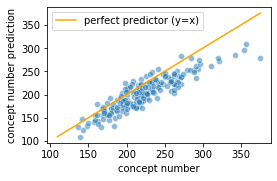
\includegraphics[height=3.5cm,width=.48\textwidth, keepaspectratio]{Figures/Ch2/metric_concept_number.png}  }
\subcaptionbox{Co-intent similarity.\label{fig:metric_cointent}}{
    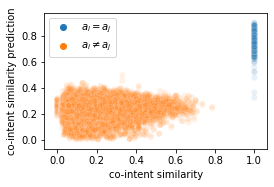
\includegraphics[height=3.5cm,width=.48\textwidth, keepaspectratio]{Figures/Ch2/metric_cointent.png}  }
\caption{Predicted metrics against the actual values, for the 200 samples with 20 objects and attributes from the test set.}\label{fig:metric}
\end{figure}

%\begin{figure}
%\centering
%\subcaptionbox{Number of concepts against size of the samples for square samples.}{\missingfigure[figcolor=white, figwidth=.48\textwidth]{Number of concepts against size of the samples?}}
%\subcaptionbox{Number of concepts upper bounds against size of the samples for non-square samples with 20 attributes.}{\missingfigure[figcolor=white, figwidth=.48\textwidth]{Number of concepts against size of the samples?}}
%\caption{Number of concepts and upper bounds against size of the FC, for a fixed density of $0.3$.}\label{fig:number-concepts}
%\end{figure}

The Pearson correlation coefficient is $0.9$ between the actual concept number and the prediction, indicating a strong correlation.
We can notice in \cref{fig:metric_concept} the tendency of the model to under-evaluate the concept number.
% and the p-value for testing non-correlation of $9.3 \times 10_{-74}$
We mention in \cref{sec:lattice-algo} a naive upper bound of the number of concept $2^{min(|O|,|A|)}$. In~\cite[p. 2]{lattice-size:2001:kuznetsov}, Kuznetsov mentions a more involved upper bound defined by Schütt:
$$3/2 \times 2^{\sqrt{|\mathbf{I}| + 1}} - 1$$
The density $d$ of the FC is such that $d = \frac{|\mathbf{I}|}{|O|\times|A|}$, so we can write $|\mathbf{I}| = d \times |O|\times|A|$.
%We show these two upper bounds compared to the actual number of concepts for the samples in our dataset and our predictions in \cref{fig:number-concepts}.
The predictions performed by our model are much smaller than the theoretical upper bounds of the number of concepts.
The prediction performance of the model is very helpful for our final goal, the generation of concepts, as mentioned in \cref{sec:boa-metric}.

When predicting the co-intent similarity, BoA manages to differentiate $a_i$ and $a_j$ when $a_i = a_j$.
However, the predictions in the other cases are not clear:
for similarities between $0$ and $0.8$, they seem randomly picked between $0$ and $0.4$.
%It appears the model has trouble learning the co-intent similarity.
The analysis of the training process reveals a small difference between the MSE of the first and the last training epochs: from $0.17$ to $0.05$.
Using MSE on values between 0 and 1 seems to cause the problem: an MSE of $0.05$ corresponds to an actual distance of around $0.22$, so 10\% of the interval of definition of co-intent similarity.
We envision several solutions, like changing the loss to \textit{mean absolute error} (MAE) or normalizing the similarity.
% In particular, normalizing and choosing a more appropriate loss could significantly improve the performance.
% We can expect that any improvement to the metric learning process would increase the quality of the embeddings.

%-> normalisation (log, exp,...) [0;1] ~> [0;inf[
%Suggestion mean-variance norm










\subsection{Experiments on Real-World Datasets}\label{sec:boa-real-world-expe}

To evaluate the performance of BoA on real-world datasets, we reproduce the link prediction and attribute clustering of~\cite{fca2vec:2019:durrschnabel}.
%
We use the same ICFCA dataset as~\cite{fca2vec:2019:durrschnabel} for link prediction.
However, for attribute clustering, we use SPECT heart\footnote{\url{https://archive.ics.uci.edu/ml/datasets/SPECT+Heart}} as it is smaller than {wiki44k}, with dimensions closer to the training data: 68 objects and 23 attributes.
Additionally, SPECT heart is much denser than wiki44k with a density of $0.23$.
Descriptive statistics on SPECT heart are reported in \cref{tab:spect}.

\begin{table}
    \centering
    \begin{tabular}{lllll}
    \toprule
    Dataset & \# Objects & \# Attributes & Density & \# Concepts\\
    \midrule
    SPECT heart & 68 & 23 & 0.23 & 911 \\
    \bottomrule
    \end{tabular}
    \caption{Descriptive statistics on SPECT heart.}
    \label{tab:spect}
\end{table}

We train the CBoW and SG variants of FCA2VEC models using the same settings as in~\cite{fca2vec:2019:durrschnabel}, with 20 random iterations of each model and an embedding size of 3.
To obtain comparable results, we reduce the embeddings produced by BoA to 3 dimensions by applying two standard dimensionality reduction techniques:
\textit{principal component analysis} (PCA) and \textit{t-distributed stochastic neighbor embedding} (TSNE).
We use Student's t-test on means to determine if the results are significant.

We report the link prediction performance in \autoref{tab:object}.
The three BoA variants show a significantly different performance from o2v SG, with all the p-values lower than $0.005$.
%
We found that the classifier based on BoA, the one with the best F1 score, systematically answers positive.
%Our TSNE variant seem performs normally however.
Additionally, we fail to reproduce the performance of~\cite{fca2vec:2019:durrschnabel} (F1 score of $0.69$ for o2v CBoW, $0.66$ for o2v SG)
Finally, the ICFCA context is very sparse: it has a density of $0.003$ on the train and $0.005$ on the test set.
Due to this, the task may not be representative of the performance of the object embeddings on most datasets.
%
These results hint that the task needs to be adapted to get proper insights into the object embedding performance.
%
%
The attribute clustering performance is reported in \autoref{tab:attribute}.
In this experiment, we find that the CBoW variant performs significantly better than the SG (all t-test p-values under $0.0005$).
This is the opposite of the result found by~\cite{fca2vec:2019:durrschnabel} for attribute clustering.
However, this result may be due to using a different dataset.
Interestingly, the BoA PCA variant performs equally to the full BoA.
The performance of BoA (and BoA PCA) is significantly better than a2v CBoW for 2 and 5 clusters (p-values under $10^{-14}$).
For 10 clusters however, a2v CBoW performs significantly better (p-value under $0.001$).
%
%Our model show a relative improment of 6\% for 2 clusters and 57\% for 5 clusters.
The model improves the performance of a2v CBoW by 4\% for 2 clusters and 8\% for 5 clusters.




\begin{table}[t]
\caption{Performance on the link prediction task (mean~$\pm$~std.).}\label{tab:object}
\centering
\begin{tabular}{lrrr}
\toprule
Model &  Precision & Recall & F1 \\
\midrule
o2v-CBoW    &  $0.63 \pm 0.05$ & ~$0.46 \pm 0.05$ & ~$0.53 \pm 0.05$ \\
o2v-SG      &  $0.70 \pm 0.04$ & $0.49 \pm 0.03$ & $0.57 \pm 0.02$ \\
\midrule
BoA PCA 3d  &  $0.65$ & $0.42$ & $0.51$ \\
BoA TSNE 3d &  $0.58$ & $0.67$ & ${0.62}$ \\
BoA         &  $0.50$ & $1.00$ & ${0.67}$ \\
\bottomrule
\end{tabular}
\end{table}


\begin{table}[t]
\caption{Performance on the attribute clustering task with 2, 5 and 10 clusters (mean~$\pm$~std.).} %(mean~$\pm$~std.)
\label{tab:attribute}
\centering
\begin{tabular}{lrrr}
\toprule
Model              & k = 2 & k = 5 & k = 10 \\
\midrule
a2v-SG             & $0.35 \pm 0.13$ &  $0.11 \pm 0.03$ & $0.042 \pm 0.010$ \\
a2v-CBoW           & $0.66 \pm 0.00$ &  ~$0.14 \pm 0.02$ & ~${0.063 \pm 0.013}$ \\
\midrule
BoA TSNE 3d & $0.30$ & $0.29$ & $0.044$ \\
BoA PCA 3d  & ${0.70}$ & ${0.22}$ & $0.051$ \\
BoA         & ${0.70}$ & ${0.22}$ & $0.051$ \\
\bottomrule
\end{tabular}
\end{table}

